\chapter{Chapter 2. Background}

In this chapter we will elaborate on the history and relevant details of the implementation of NLDAS and Noah-LSM, frame the problem in terms of the difference between numerical modeling and data-driven modeling approaches, and describe the technical properties and pertinent considerations for neural networks intended for time series modeling.

\section{NLDAS and Noah-LSM: History and Implementation}

\begin{figure}[h]
    \centering

    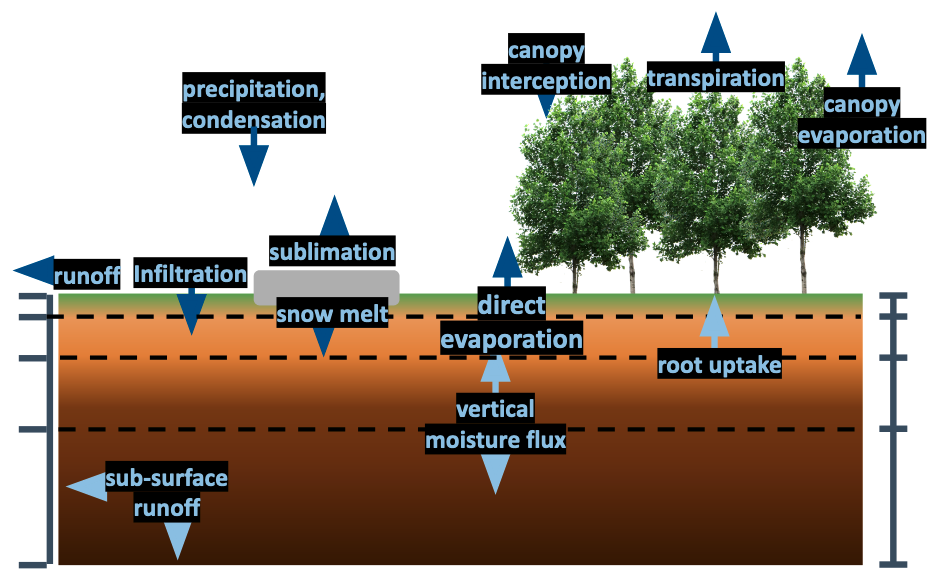
\includegraphics[width=.66\linewidth]{figures/schematic_noah-overview.png}

    \caption{Schematic diagram of the feedbacks contributing to the evolution of soil moisture in Noah-LSM}
    \label{noah-schematic}
\end{figure}

The theoretical framework underpinning Noah-LSM was initially formulated in the 1980s as part of the OSU model, which characterizes boundary layer moisture and energy fluxes as a 2-layer soil model subject to atmospheric forcings. The model expresses the infiltration and movement of water between the soil layers with the diffusive form of the Richards equation \citep{mahrt_two-layer_1984}, direct evaporation using an analytic approximation of the Penman-Montieth relation in terms of atmospheric stability \citep{mahrt_influence_1984}, and basic plant transpiration in terms of vegetation density and soil water content \citep{pan_interaction_1987}. These features form an interdependent system of differential equations that are numerically integrated using a combination of the Crank-Nicholson method and finite-differencing \citep{chen_impact_1997}, which introduces the need for short time steps of 15 or 30 minutes in order for the system to remain numerically stable \citep{cartwright_dynamics_1992}\citep{mahrt_two-layer_1984}.

The OSU model was later significantly improved, renamed to the first generation of Noah-LSM, and coupled with the NCEP Eta forecast model. Noah-LSM expanded the domain to four soil layers of increasing thicknesses (10cm, 30cm, 60cm, and 100cm), improved runoff dynamics by implementing Philip's equation for infiltration capacity \citep{schaake_simple_1996}, and represented the influence of soil texture on moisture transport by introducing bounds on bare-soil potential evaporation that are determined by the soil composition \citep{betts_assessment_1997} \citep{mahfouf_comparative_1991}. The model also features a significantly enhanced representation of vegetation including a more thorough treatment of canopy resistance via a ``Jarvis-type'' model of leaf stomatal control \citep{jarvis_interpretation_1976} \citep{jacquemin_sensitivity_1990}, which accounts for the dependence of transpiration on insolation, air temperature and dewpoint, soil moisture content, and vegetation density. The vegetation effects are scaled by a monthly climatology of normalized difference vegetation index (NDVI) values observed by the NOAA-AVHRR satellite radiometer, which serve as a proxy for green vegetation fraction (GVF) \citep{gutman_derivation_1998} \citep{chen_modeling_1996}, and the depth of root water uptake associated with plant transpiration is determined by a pixel's vegetation class as specified by the Simple Biosphere Model \citep{dorman_global_1989}. Finally, the model's utility was greatly expanded with the addition of a frozen soil and snow pack parameterization incorporating the thermal and hydraulic properties of fractionally-frozen soil layers, the effects of state changes \citep{koren_parameterization_1999}, radiative feedbacks from partial snowpack coverage, and a snow density scheme \citep{ek_implementation_2003}.

Soon after the turn of the millennium, the first generation of NLDAS was under development as part of a multi-institution collaborative effort sponsored by the Global Energy and Water Cycle Experiment (GEWEX) Continental-scale International Projects (GCIP) team. The goal of the project was to incorporate long-term observations of land surface temperature, snow pack depth, and meteorological forcings from multiple sources (in-situ, satellite, radar) into a common framework used to independently evaluate land surface states and energy fluxes with four land surface models including Noah-LSM \citep{mitchell_multi-institution_2004}. Over a domain including the full conterminous United States (CONUS) at $0.125^\circ$ resolution, the models were allowed to spin up over the course of a year, and soil states were recurrently used to initialize subsequent time steps rather than being ``nudged'' to correct for drift. Land cover and soil texture classification over the domain was derived by coarsening the University of Maryland and STATSGO datasets, respectively, from their native 1km resolutions \citep{hansen_global_2000}, surface geometry and elevation is provided by the GTOPO30 dataset \citep{earth_resources_observation_and_science_centeru_s_geological_surveyu_s_department_of_the_interior_usgs_1997}, and the parameter values for soil hydraulic properties were adapted from observations taken at the University of Virginia \citep{cosby_statistical_1984}.

\begin{table}
    \centering
    \begin{tabular}{ l l l l l}
        Forcing & Unit & Source & $\Delta$t & $\Delta$x \\
        \hline
        \multirow{2}{*}{Precipitation} & \multirow{2}{*}{kg m$^{-2}$} & CPC Gauge observations & 24h & 14km \\[-12pt]
        & & WSR-88D retrievals & 1h & 4km \\
        Temperature & K & NCEP NARR & 3h & 32km \\
        Specific Humidity & kg kg$^{-1}$ & NCEP NARR & 3h & 32km \\
        Surface Pressure & Pa & NCEP NARR & 3h & 32km \\
        Wind Velocity & m s$^{-1}$ & NCEP NARR & 3h & 32km \\
        Incident LW Flux & W m$^{-2}$ & NCEP NARR & 3h & 32km \\
        Incident SW Flux & W m$^{-2}$ & GOES, NARR & 3h, 1h & 14km \\
        Green Veg Fraction& \% & AVHRR NDVI & Monthly & 16km \\
        Leaf Area Index & m$^2$ m$^{-2}$ & UMD, AVHRR NDVI& Monthly & 16km \\
        Snow Water Equivalent & kg m$^{-2}$ & Noah-LSM & 14km \\
    \end{tabular}
    \caption{Atmospheric forcings and other time-varying parameters provided by NLDAS-2 at a 1-hourly resolution on the $0.125^\circ$ CONUS grid. Data are resampled using spatial bilinear interpolation, then temporal disaggregation according to \citep{cosgrove_real-time_2003}. NLDAS forcing files also include values for convective available potential energy, the ratio of precipitation from convection, and surface potential evaporation (calculated as in \citep{mahrt_influence_1984}), but these three values aren't currently used as inputs to the models. Snow water equivalent estimates are an output of Noah-LSM by default, but are included as a predictor here under the assumption that they can be provided from a separate model or data assimilation source.}
    \label{forcing}
\end{table}

Attention remained on Noah-LSM in the following years as it continued to support NLDAS and other data assimilation and forecasting systems, which led to a series of improvements introduced alongside the next phase of the NLDAS project. A seasonal effect was added to vegetation by scaling the leaf area index (LAI) by the GVF within bounds determined by the plant type, and transpiration was scaled by a root uptake efficiency factor determined by the proximity of soil temperature to an optimum growth temperature (298 K). Several parameters were adjusted including the influence of vapor pressure deficit on transpiration rate, the minimum stomatal resistance for several plant species, and hydraulic parameters for some soil textures. The aerodynamic conductance coefficient -- an important factor in the strength of moisture and energy fluxes from the surface -- was increased during daylight hours, and a basic anisotropy model was introduced by modifying the albedo of some surfaces in terms of the solar zenith angle \citep{wei_improvement_2011}. Snowpack physics were also modified to improve surface exchange coefficients, and to gradually diminish the snow albedo over the time since the last snowfall \citep{livneh_noah_2010} \citep{liang_simple_1994}. These changes introduce new feedbacks and involve sensitive parameters like LAI which have a strong influence on the model's dynamics \citep{rosero_quantifying_2010}. The retrospective NLDAS-2 data record generated after applying these modifications extends back to 1979, and continues to be updated in a near real-time capacity \citep{xia_continental-scale_2012}.

The NLDAS-2 time-varying retrospective forcings listed in Table \ref{forcing} will serve as the predictors used by the neural networks to forecast the Noah land surface model soil moisture states. Temperature, humidity, pressure, wind speed and heading, and longwave flux are derived exclusively from the National Centers for Environmental Prediction (NCEP) North American Regional Reanalysis (NARR) data product. As part of the downscaling procedure from their native 32km resolution to the 1/8$^\circ$ NLDAS domain, a lapse rate adjustement is applied to the temperature and humidity fields based on the elevation profile. Downward shortwave radiative flux is calculated using a blend of NARR and hourly Geostationary Operational Environmental Satellite (GOES) data, with a ratio-based bias correction based on \citep{berg_impact_2003} applied to account for a known positive bias in NARR-reported downward shortwave flux, and to mitigate discontinuities arising from the merger the two data sources \citep{pinker_surface_2003} \citep{xia_continental-scale_2012-1}. Precipitation receives a special treatment in order to ensure sufficient spatial resolution and consistency; the Climate Prediction Center (CPC) daily gauge-based product \citep{chen_assessing_2008} serves as the baseline, which is temporally disaggregated to 1 hour resolution using National Weather Service WSR-88D radar retrievals \citep{fulton_wsr-88d_1998}. In regions lacking radar coverage, the disaggregation is completed using a weighted combination of the CPC's satellite-derived estimates from morphed passive-microwave and infrared observations (CMORPH) \citep{joyce_cmorph_2004}, and the CPC Hourly Precipitation Dataset (HPD), with NARR data as a final fallback \citep{baldwin_ncep_1997}.  Although both the LAI and GVF vegetation parameters are based on multi-year monthly averages, they are disaggregated to an hourly resolution in order to be smoothly variable \citep{wei_improvement_2011}, and are thus treated like an atmospheric forcing in this work.

\section{Calibration and Validation of Noah-LSM}

During the development of Noah-LSM, researchers integrated information from a variety of observational datasets in order to calibrate and validate the soil moisture, energy flux, and radiative components of the model outputs. The initial field campaign data that bootstrapped development of the OSU model precursor came from the First International Satellite Land Surface Climatology Project Field Experiment (ISLSCP FIFE) \citep{sellers_overview_1992}, which utilized averaged evaporation data data from 10 stations in a 15x15km grassland area during the warm season of 1987. The OSU model showed strong performance in capturing the seasonal and diurnal cycle of evaporation, soil moisture, heat fluxes, and skin temperature, however struggled during wet periods due to an over-estimation of evaporation caused by the canopy resistance formulation \citep{chen_modeling_1996}.

Based on these results, others utilized further observations to integrate and parameterize new processes within Noah-LSM in order to mitigate the shortcomings. For example, and the bare surface evaporation and vegetation schemes were improved by \citep{betts_assessment_1997} based on four 48-hour intensive observation periods within FIFE, surface runoff parameters were improved by \citep{schaake_simple_1996} based on long-term USGS stream discharge datasets from gauged basins in Oklahoma, Mississippi, and North Carolina. The radiation balance and heat flux magnitudes from Noah-LSM were evaluated with respect to a full year of data from 7 sites in the Oklahoma Mesonet by \citep{sridhar_validation_2002}, who found a slight positive bias in flux magnitudes, but overall good performance with root mean squared error rates for all fluxes falling below 2.5 $MJ\,m^{-2}\,d^{-1}$. Fluxes, temperatures, radiation, and soil moisture were further validated by \citep{robock_evaluation_2003} with respect to Oklahoma Mesonet and ARM/CART surface station observations from 1998 and 1999; they found that Noah-LSM performed better than all other models in the NLDAS framework, but had a positive bias in soil moisture around 7\%, which was postulated to be the consequence of inadequacy in the static soil parameterization.

Snow and frozen soil posed a particular issue during the early development of Noah-LSM, as neglecting the physics of partially-frozen soil, fractional snow cover, and variable snow density resulted in significant underestimates in soil moisture, and high error rates in soil temperature. These shortcomings were addressed by the new physics introduced by \citep{koren_parameterization_1999}, which were calibrated based on soil moisture, temperature, and snow water equivalent observations from Rosemont, Minnesota during the 1995-1996 cold season. The ~20\% under-estimation of lower-layer soil moisture and high error in soil temperature were greatly diminished as a consequence of the changes. Significant snowpack volume under-estimates were also addressed by \citep{livneh_noah_2009} using SNOTEL station snow water equivalent data, and subsequently by \citep{barlage_noah_2010} based on problems noted by \citep{pan_snow_2003} using both SNOTEL and SNODAS data. In combination, these process improvements reduced the low bias to about 15\%, and improved the snow water equivalent correlation with the observations to about 80\%.

In the lead-up to the second generation of NLDAS, \citep{wei_improvement_2011} implemented further improvements to warm-season processes which were validated based on ARM/CART surface flux stations as well as GOES satellite retrivals of land surface temperature during the 1998 and 1999 warm seasons. The consequence was a reduction in spring-season positive bias in latent from 80 $W\,m^{-2}$ to about 20 $W\,m^{-2}$ and land surface temperature with a correlation of about .85, a slight negative bias of $-1.26\,K$, and root mean squared error around $3.08\,K$. Additionally, \citep{xia_evaluation_2014} validated NLDAS-2 modeled soil moisture against 20 years of monthly data from the Illinois climate network (1986-2004), 6 years of daily data over 72 sites from the Oklahoma Mesonet (1997-2002), and 8 years of daily data from 121 SCAN sites (2002-2009). They found that Noah exhibited a mean monthly anomaly correlation of .82 in the first 2m, which was stronger in the warms seeason but struggled when the ground was frozen or snow was present, especially in lower two soil layers. The daily mean anomaly correlation from the Oklahoma Mesonet data was greater than .8 in the lower layers and .77 in the surface layer, while the monthly averages were all above .85 with about 15\% relative MAE and a relative bias around -15% for all three tested layers. Regional analyses with respect to the widely-dispersed SCAN stations indicate substantial variability in performance; Noah-LSM struggled with the surface layers in the Northeast US with a correlation of only about .2, but was consistently better than .5 correlation elsewhere, especially in the Great Plains and Northwest. The midwest also exhibited a large dry bias, which is likely the consequence of a lack of irrigation information in the cropland-dominated region.

Finally, an entropy-based decomposition of uncertainty was employed by \citep{nearing_benchmarking_2016} to quantify the components of error in Noah-LSM caused by improper characterization of forcings, model dynamical structures, and model parameters. By comparing to soil moisture observations from 49 SCAN sites and 50 AmeriFlux stations active between 2001 and 2011, they determined that inadequate model parameters like soil texture and vegetation classification were the greatest sources of uncertainty in the soil moisture profile, while biased input forcings were the dominant cause of uncertainty for energy fluxes.

\section{Distinctions in Modeling Techniques}

\begin{figure}[h]
    \centering

    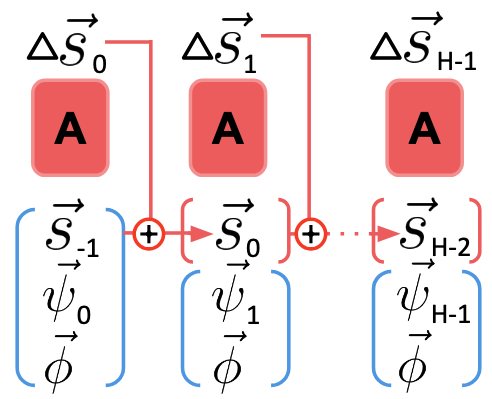
\includegraphics[width=.66\linewidth]{figures/schematic_scann.png}

    \caption{Diagram of a self-cycling discrete-time dynamical system with no hidden state. At each time, nonlinear operator \textbf{A} maps an initial state $\vec{s}_{k-1}$, exogenous forcing $\vec{\psi}_k$, and time-invariant parameters $\vec{\phi}$ to a new state $\Delta \vec{s}_k$, used to initialize the subsequent time step, and so forth until $H$ predictions have been made.}
    \label{scann}
\end{figure}

\subsection{Noah-LSM as a Discrete Dynamical System}

At its core, Noah-LSM is a collection of coupled differential equations that express the total derivative of land surface states $\frac{d\vec{s}}{dt}$ in terms of the current state $\vec{s}$, forcing $\vec{\psi}$, and time-invariant properties of each grid cell $\vec{\phi}$. Since the model is implemented as an algorithmic procedure and is not continuously differentiable, we will use the notation $\frac{\Delta \vec{s}_k}{\Delta t} \approx \mathbf{A}(\vec{s}_{k-1}, \vec{\psi}_k, \vec{\phi}, \Delta t)$ to refer to the model as a transition function evaluated at a discrete time step $\Delta t$, such that the system evolves as a dynamical system described by Equation \ref{dynamical}.

\begin{equation}\label{dynamical}
    \vec{s}_k = \vec{s}_{k-1} + \mathbf{A}(\vec{s}_{k-1}, \vec{\psi}_k, \vec{\phi}_k, \Delta t) \cdot \Delta t
\end{equation}

Here, $\vec{s}_k$ refers to the model's dynamic state variables like snow pack depth, soil moisture and temperature, and canopy storage, $\vec{\psi}_k$ encodes the covariate atmospheric variables from Table \ref{forcing} (which are derived from weather forecasts or observations), and $\vec{\phi}$ includes time-invariant coefficients of the governing equations like vegetation type/fraction, soil texture, and slope/elevation. As a matter of convention, the time step $k=0$ refers to the first perturbation of the initial state after applying the model's first increment change estimate, and includes the forcings that informed that perturbation, consistent with the relationships depicted by Figure \ref{scann}.

To generate a time series, Noah-LSM numerically integrates the system of equations using Euler and Crank-Nicholson techniques, which explicitly evaluate the differential equations at several time intervals per computational time step in order to estimate the nonlinear change in state, which evolves continuously in the real system being modeled. It is crucial that the increment change in time remains small between evaluations of the model (15min for NLDAS-Noah) to mitigate truncation error from the assumption of local linearity \citep{mitchell_multi-institution_2004} \citep{cartwright_dynamics_1992}. As Figure \ref{scann} suggests, the model does not retain any ``hidden'' internal information that is updated between timesteps; at each point, the information available to determine the new change in state is limited to the input domain of the model.

\subsection{Process-based vs Data-driven Models}

The process-based approach of numerical models like Noah-LSM is practically and epistemologically distinct from data-driven techniques like deep learning. In a process-based paradigm, the inductive biases that govern the model's behaviors can be explicitly understood since they are based on a characterization of the physical system which is derived from theoretical knowledge. Some uncertainty is introduced by the input data, and is shared among all model types; this includes uncertainty from noise and interpolation of forcing observations, discrete treatment of surface types, etc. Aside from that, model error in process-based models arises from sources including inadequacy of the theory for describing the system (that is, phenomena which are neglected or misrepresented, and become a source of unexplained variance), and truncation error accumulated from the approximation techniques used to solve the model's governing equations. Explicit understanding of the reasons for the model's behavior has the advantage of being interpretable, in the sense that particular systems within the model can be independently evaluated and blamed for contributing uncertainty. Additionally, granting the ability to impose absolute constraints within the model structure ensures the outputs fully adhere to some physical requirements, such as conservation of water and energy. Nonetheless, the onus falls entirely on the model developer to adjust many details of the implementation of the processes. The act of tuning a numerical model's parameters often implies postulating a source of uncertainty, addressing it by manually manipulating coefficients or introducing new systems within the governing equations, and then evaluating the impact of the changes using correlational analysis with a subset of the available data. This can be a laborious process, and typically results in the gradual accumulation of feedbacks and complexity within the model.

In contrast, many data-driven approaches to modeling physical systems -- deep learning in particular -- sacrifice the explainability and rigorous physicality of their estimates in exchange for developing a statistically optimal approximation of the relationship between the input and output domains by any means available. Although the overall algorithmic structure of the ANN is established by the developer -- typically based on broad heuristics from past literature and experimentation -- very little control can be asserted over the particular means by which predictions are determined from inputs. Instead, the effectiveness of the ANN's performance is characterized in terms of a differentiable loss function (also known as the objective or cost function) which may be defined by the developer, and which is fundamentally (though indirectly) important for determining the solution developed in the training phase.

An ANN's learnable parameters refer to the real-valued elements of a series of arbitrarily-sized square matrices encoding affine transformations. Each ``layer'' of the ANN is comprised of one of these affine transformations followed by an element-wise nonlinear operation on its output, and the full ANN typically consists of multiple layers which are combined via composition or any kind of differentiable arithmetic operation. During training, all of the ANN's learnable parameters are iteratively adjusted by estimating the gradient of the loss function with respect to the parameters (given batched subsets of the predictor/target data pairs) then determining the direction and magnitude by which the parameters in each of the layers should be modified with an algorithm called backpropagation \citep{rumelhart_learning_1986}. The general strategy of determining the sensitivity of the loss landscape to changes in the ANN's parameters, and tweaking them accordingly, is referred to as gradient descent. Given at least 2 layers (which constitutes the definition of a \textit{deep} ANN), the network is theoretically capable of expressing an arbitrary decision boundary or multivariate function given a sufficient number of parameters \citep{hornik_multilayer_1989}. This high level of expressivity enables the network to learn complex relationships and generalizations among high-dimensional parameters, given repeated exposure to instances of these relationships during training.

The principle of ANNs using high-dimensional nonlinear correlations rather than explicit processes to model the correspondence between two datasets is powerful because they can approximate a highly nonlinear regression without numerically integrating a complex algorithm, and they can learn their parameterization based on a large volume of data without manual intervention. The quintessential drawback of relying on a black-box approach, though, is that models may perform poorly for no apparent reason, or may perform well for a fraught reason. For example, in one commonly-invoked anecdote described by \citep{lapuschkin_unmasking_2019}, an image classifier over-performing but failing to generalize at identifying horses in a grassy field was found to actually rely on the presence of the watermark of a particular equestrian photographer whose work was a part of the training data. As such, only regarding bulk statistics and loss performance as indicative of a model's success is insufficient to consider it trustworthy. In a data-driven paradigm, then, the role of the ANN developer is to facilitate effective and reliable learning through careful training data curation, congnizant loss function and model architecture design, and thorough evaluation of the model's behavior in local and global scenarios throughout the input domain in order to ensure the effectiveness and consistency of predictions in a variety of inference settings.

Furthermore, it is important to note that in the current scope of this work, it is not possible for the ANNs to leverage their expressivity to out-perform the numerical model. Since the ANNs presented here are merely emulating the processes that are programmed into Noah-LSM, it isn't reasonable to expect the models to form a more accurate representation of real soil dynamics. Nonetheless, it is conceivable that future work could utilize a similar approach to \citep{o_global_2021} in order to integrate observational data into the training domain alongside model data, or to use it as a prediction target. The merger of these two data sources could aid in improving a data-driven model beyond the limitations of a numerical model's structure.

\section{Deep Learning of Time Series}

\begin{figure}[h!]
    \centering

    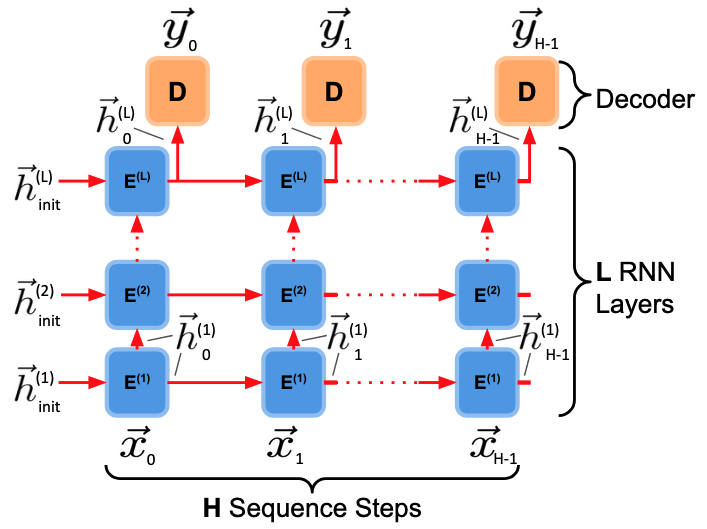
\includegraphics[width=.95\linewidth]{figures/schematic_abstract-rnn.png}

    \caption{Schematic representation of an abstract sequence-to-sequence RNN with multiple layers.}
    \label{schematic-rnn}
\end{figure}

The most simple variant of an ANN is referred to as a feed-forward neural network (FNN), which consists of a series of composed layers (see previous section) mapping the input vector directly to the output. Although a FNN is theoretically capable of simulating Noah-LSM in the manner of Figure \ref{scann}, inductive biases are commonly introduced in model architectures in order to promote efficiency, explainability, stability, and parsimony. For example, most neural networks used for sequence modeling like the recurrent neural networks (RNNs) in Figure \ref{schematic-rnn} maintain one or more ``hidden'' latent parameters $\vec{h}$ with an arbitrary number of dimensions. This vector is modified and passed along by each subsequent iteration, giving the network the ability to make temporal generalizations and propagate information to future predictions. Although $\vec{h}$ is typically difficult to interpret directly, the gradient descent process incentivizes the network to preserve and consolidate information that is needed to accurately generate the full sequence of predictions. This construct is promising for improving the models' ability to estimate soil dynamics because characteristic drydown curves are known to exhibit hysteresis depending on their recent patterns of wetting and drying \citep{haines_studies_1930}. %Each of the following network architectures ultimately aim to improve the information quality of the latent vector by implementing algebraic structure, introducing statistical uncertainty, and encouraging sparsity.

\begin{equation}\label{eq_rnn}
    \begin{split}
        %\vec{h}_k^{(1)} &= \mathbf{E^{(1)}}\left(\vec{h}_{k-1}^{(1)},\, \vec{\psi}_k,\, \vec{\phi}\right) \\
        \vec{h}_k^{(1)} &= \mathbf{E^{(1)}}\left(\vec{h}_{k-1}^{(1)},\, \vec{x}_k\right) \\
        \vec{h}_k^{(j)} &= \mathbf{E^{(j)}}\left(\vec{h}_{k-1}^{(j)},\, \vec{h}_k^{(j-1)}\right) \\
        \vec{y}_k &= \mathbf{D}\left(h_k^{(L)}\right)
        %\vec{s}_{k+1} &= \vec{s}_{k} + \mathbf{D}\left(h_k^{(L)}\right)
    \end{split}
\end{equation}

The RNNs discussed here will follow the general structure described by Equation \ref{eq_rnn}, which is consistent with the abstract architecture diagrammed in Figure \ref{schematic-rnn}, and follows the typical approach for constructing RNNs as outlined in \citep{russell_artificial_2020}. The architecture consists of L encoder layers (\textbf{E}$^{(1)}$-\textbf{E}$^{(L)}$) which generate H top-layer latent vectors corresponding to each of the prediction times, and 1 layer of decoder weights \textbf{D} which converts each of the top-layer latent vectors to a prediction for the increment change in state $\Delta \vec{s}$ between the current timestep and the next one. Parameters for \textbf{E} and \textbf{D} are shared across timesteps, however each of the L layers have distinct parameters. Here, $\vec{h}_k^{(1)}$ is a member of the time series of first-layer latent vectors given the arguments $\vec{x}_k$ and the latent vector from the previous first-layer timestep $\vec{h}_{k-1}^{(1)}$. Moving upward, $\vec{h}_k^{(j)}$ is an intermediate-layer latent vector such that $j \in [2,\,L]$, and when $k=0$ (the first horizon timestep), $\vec{h}^{(s)}_{-1} = \vec{h}^{(s)}_{\text{init}}$ for any layer $s$. In many cases, the initial hidden states $\vec{h}^{(s)}_{init}$ are randomized or set to zero, however in this project we use a separate spin-up RNN to establish them, as will be discussed in the Methodology section.

\begin{figure}[h!]
    \centering

    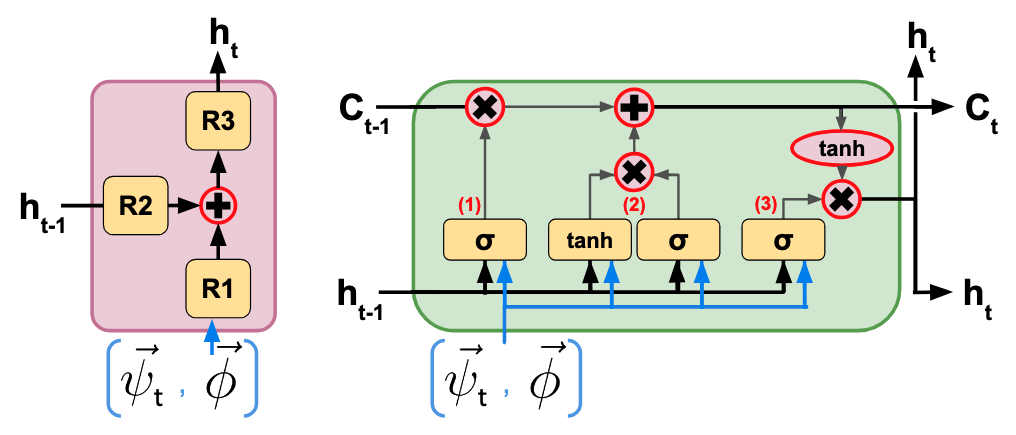
\includegraphics[width=.95\linewidth]{figures/schematic_rnns-both.png}

    \caption{Schematic representation of individual RNN cells, the na\"ive RNN (left), and the LSTM (right)}
    \label{rnns-both}
\end{figure}

The term RNN does not refer to a specific neural network architecture, but rather the category of architectures that share their weights across sequence steps. The sub-network unit of weights applied at each timestep (\textbf{G} or \textbf{E} in Figure \ref{s2s-default}) is referred to as a RNN cell, and must contain internal structure for converting inputs from lower layers and the previous timestep into an output. Unlike traditional ANNs which use backpropagation to train on single input-output pairs, each cell must balance the penalty of its loss gradient between contributions from the input at each timestep with contributions from the latent vector of the previous timestep. To accommodate this difference, RNNs are trained using a special type of gradient descent called backpropagation through time, which balances the loss with respect to the two input sources, and accumulates it across all timesteps before updating each cell's parameters.

The most basic form of the RNN architecture (diagrammed on the left side of Figure \ref{rnns-both}) consists of 3 separate affine operations. As shown in the figure, R1 and R2 convert the lower-layer and previous-timestep vectors, respectively, into two uniformly-sized internal latent vectors. The sum of these internal vectors are transformed by a third affine operation, R3, into the cell's output, which is passed along to the higher layer and subsequent steps within the same layer.

This style of na\"ive RNN is vulnerable to the so-called vanishing or exploding gradient problem, which arises from the fact that the cell output is the direct product of learned matrix operations. Since during training each cell's weights are updated recurrently based on many sequence steps, the loss gradient with respect to each learned parameter can become incredibly sensitive to changes in each parameter. This can cause weights to become very close to zero, or to diverge to very large numbers, which halts the learning process \citep{mozer_focused_1995}. Furthermore, since the latent state passed between sequence steps undergoes a nonlinear transformation at each instance of the cell, it is more tenuous for the network to sustain information over a long context of past observations.

The LSTM architecture addresses these shortcomings by maintaining a separate hidden state $\vec{C}_t$ called the context vector. Rather than being generated by a matrix operation at each step, the context vector is only modified from the previous step's value using the output of a series of three ``gates.'' These gates (numbered in Figure \ref{rnns-both})  include (1) the ``forget gate'', which uses a FNN to select a vector of values in the range (0,1). The forget vector is multiplied element-wise by $\vec{C}_{t-1}$ in order to selectively emphasize or diminish its activation. The ``update gate'' (2) transforms the inputs into a new coefficient vector in the range (-1,1), which is added to the context vector in order to retain information from the current time step. Finally, the ``output gate'' (3) generates a vector of multiplicative coefficients in the range (0,1) used to scale the new context vector $\vec{C}_t$ to the output latent state $\vec{h}_t$ \citep{hochreiter_long_1997}. The context vector remains stable compared to a hidden vector that is recurrently operated on by the same weight matrix, which facilitates the network to learn over a longer sequence interval.

The Transformer architecture has dominated many sequence modeling tasks in recent literature thanks to the key innovation of multi-head self-attention (MSA), which enables the architecture to learn complicated relationships between individual members of the input sequence regardless of their relative position. Additionally, transformers are efficient to train in parallel, unlike RNN architectures which rely on a chain of sequential operations, which makes them straightforward to train on a massive scale \citep{vaswani_attention_2017}. The results for natural language processing (NLP) \citep{devlin_bert_2019} and image classification \citep{dosovitskiy_image_2021} tasks are impressive, however there are several key drawbacks that make them less appealing for a time series generation task like this one.

First, the memory cost of a transformer scales quadratically with sequence length since MSA learns parameters relating every possible combination of input steps. This is compounded with the fact that the full input sequence needs to be re-initialized with every step during inference. These properties are a direct trade-off with the Transformer's ability to train separate sequence steps in parallel. Furthermore, unlike RNNs and CNNs, Transformers don't have an inherent notion of order. In problems like NLP where sequence position conveys some information, a simple form of locality is introduced by adding a positional embedding vector directly to the inputs. Prior literature shows that transformers equipped with positional embedding still perform no better on basic time series forecasting tasks than a simple 2-layer FNN \citep{zeng_are_2022}. For these reasons, although MSA is a very powerful tool for many applications, we will be neglecting this very popular architecture in this work.
